\section[VAN]{VAN}
	\begin{equation}
	\label{eq:van}
	\begin{split}
 		w = - C_0 + \sum_{k=1}^n \frac{CF_k}{(1+r)^k}
	\end{split}
	\end{equation}
	Consideriamo, quindi, il valore del \ac{VAN} su $12$ flussi di cassa (\textit{cashflow}), corrispondenti alle stime sull'utile realizzato alla fine di ogni mese ed un \textbf{tasso di sconto} $r$ pari al \textbf{\ac{WACC}} (\ref{eq:wacc_tax_value}).\newline
	La formula (\ref{eq:van}) diventa, quindi:	
	\begin{equation}
	\label{eq:van_caso_studio}
	\begin{split}
 		w = - C_0 + \sum_{k=1}^{12} \frac{CF_k}{(1+0,058)^k}
	\end{split}
	\end{equation}	
	Il valore $C_0$ corrisponde all'investimento iniziale del nostro progetto, quindi, pari al \textbf{CAPEX} $ 56\thinspace 170,20 \: \mbox{\euro}$.
	Assumiamo, inoltre, che i flussi mensili siano costanti nell'arco di un anno, quindi la quantità $CF_k$ non è più legata al k-esimo mese, si può esprimere, quindi, come $CF$:
	\begin{equation}
	\label{eq:flussi_cassa_mensili}
	\begin{split}
 		CF = \underbrace{x}_{fatturato \: mensile} - \underbrace{60\thinspace 131,27}_{OPEX}
	\end{split}
	\end{equation}	  	
la (\ref{eq:van_caso_studio}) diventa (il VAN diventa funzione dei flussi di cassa lordi $x$ quindi $w = y(x)$):	
	\begin{eqnarray}
	\label{eq:van_caso_studio_2}
 		y(x) & = & - 56\thinspace 170,20 + \sum_{k=1}^{12} \frac{x - 60\thinspace 131,27}{(1+0,0058)^k} \nonumber \\
 		 & = & -56\thinspace 170,20 + (x - 60\thinspace 131,27) \cdot \underbrace{\sum_{k=1}^{12} \frac{1} {(1+0,0058)^{k}}}_{{}=8,47654} \nonumber \\
 		 & = & -56\thinspace 170,20 + (x - 60\thinspace 131,27) \cdot 8,47654 \nonumber \\
 		 & = & -565\thinspace 875,32 + 8,47654 \cdot x 		
	\end{eqnarray}  		

 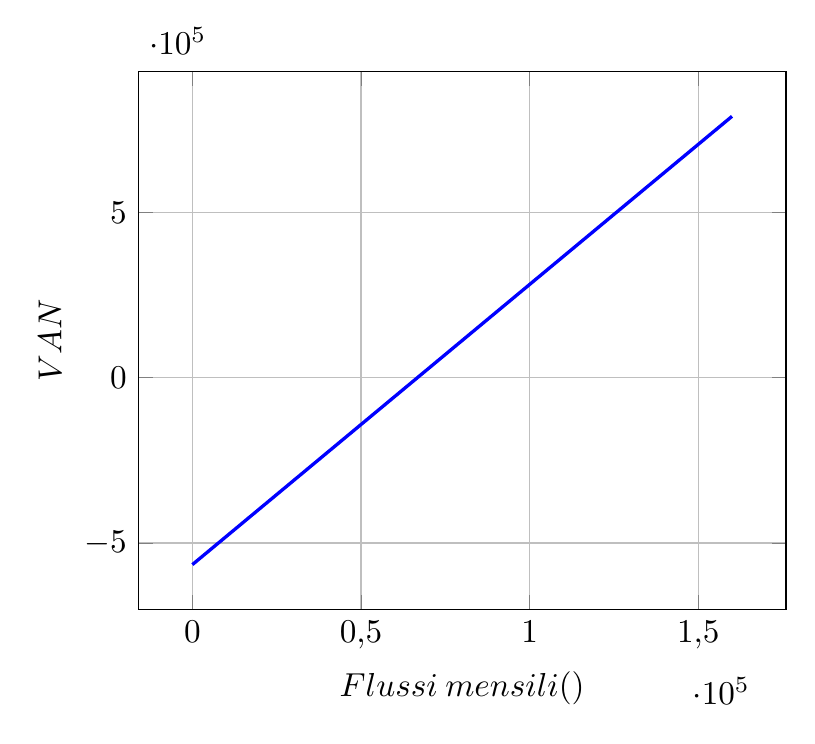
\begin{tikzpicture}[scale=1.2]
 \pgfkeys {
			/pgf/number format/.cd,
			set decimal separator={,{\!}},
			set thousands separator={}}
	\begin{axis}[ xlabel=$Flussi\: mensili (\mbox{\euro})$, 
				   ylabel=$VAN$, 
				   grid=major ]
		
		\addplot[domain=0:160000, color=blue, line width=1pt]{8.47654 * x - 565875.32};
		
	\end{axis}
\end{tikzpicture}

Un punto importante della funzione (\ref{eq:van_caso_studio_2}) è quello per cui il $ VAN = 0 $, ovvero:

	\begin{equation}
	\label{eq:van_zero}
	\begin{split}
 		y(x) = 0
 	\end{split}
	\end{equation}

Il valore $x$ per cui (\ref{eq:van_zero}) è soddisfatta 
	\begin{equation}
	\label{eq:van_pareggio_1}
	\begin{split}
 		8,47654 \cdot x - 565\thinspace 875,32 = 0	
 	\end{split}
	\end{equation}
è pari a:
	\begin{eqnarray}
	\label{eq:van_pareggio_2}
		x & = & \frac{565\thinspace 875,32	}{8,47654}	 	\nonumber \\[1.5ex] 
		  & = &  66\thinspace 757,82 \: \mbox{\euro} 
	\end{eqnarray}
Il valore di $x$ rappresenta, da un punto di vista fisico, il flusso minimo di cassa mensile affinchè il progetto risulti remunerativo alla fine del periodo in esame (12 mesi nel caso di studio proposto). \newline
Considerando il fatturato mensile pari a (\ref{eq:van_pareggio_2}), gli utili saranno pari a:
	\begin{equation}
	\label{eq:flussi_netti}
	\begin{split}
 		66\thinspace 757,82 \: \mbox{\euro} - \underbrace{60\thinspace 131,27 \: \mbox{\euro}}_{OPEX} = 6\thinspace 626,55 \: \mbox{\euro}	
 	\end{split}
	\end{equation}
fissando un tasso di sconto pari a (\ref{eq:wacc_tax_value}), si può osservare la seguente situazione:
%
%	Tabella relativa alla valutazione VAN = 0,00
%
\begin{savenotes}
\begin{table}[htb]
\centering
 \caption{VAN (Fatturato Mensile pari a $\mbox{\euro \:66\thinspace 757,82}$)}
 \begin{tabular}{p{7cm}D{,}{,}{7.2}D{,}{,}{7.2}D{,}{,}{7.2}}
 \toprule
 	\multicolumn{1}{c}{\textbf{Mese}} & \multicolumn{3}{c}{\textbf{Flussi di cassa (\euro)}} \\
 	& \multicolumn{1}{c}{Netti (\euro)} & \multicolumn{1}{c}{Attualizzati (\euro)} & \multicolumn{1}{c}{Totale (\euro)} \\
 \midrule
 	\makebox[7cm][r]{\textbf{Investimento Iniziale (CAPEX)}} & & & -56\thinspace 170,20 \\
 \midrule
 	\makebox[7cm][r]{Gennaio} & 6\thinspace 626,55 & 6\thinspace 263,28 & -49\thinspace 906,92\\ 
 	\makebox[7cm][r]{Febbraio} & 6\thinspace 626,55 & 5\thinspace 919,92 & -43\thinspace 987,00\\
 	\makebox[7cm][r]{Marzo} & 6\thinspace 626,55 & 5\thinspace 595,39 & -38\thinspace 391,60\\ 
 	\makebox[7cm][r]{Aprile} & 6\thinspace 626,55 & 5\thinspace 288,65 & -33\thinspace 102,95\\
 	\makebox[7cm][r]{Maggio} & 6\thinspace 626,55 & 4\thinspace 998,72 & -28\thinspace 104,23\\ 
 	\makebox[7cm][r]{Giugno} & 6\thinspace 626,55 & 4\thinspace 724,69 & -23\thinspace 379,54\\
 	\makebox[7cm][r]{Luglio} & 6\thinspace 626,55 & 4\thinspace 465,68 & -18\thinspace 913,86\\ 
 	\makebox[7cm][r]{Agosto} & 6\thinspace 626,55 & 4\thinspace 220,87 & -14\thinspace 692,99\\
 	\makebox[7cm][r]{Settembre} & 6\thinspace 626,55 & 3\thinspace 989,48 & -10\thinspace 703,50\\ 
 	\makebox[7cm][r]{Ottobre} & 6\thinspace 626,55 & 3\thinspace 770,78 & -6\thinspace 932,73\\
 	\makebox[7cm][r]{Novembre} & 6\thinspace 626,55 & 3\thinspace 564,06 & -3\thinspace 368,67\\ 
 	\makebox[7cm][r]{Dicembre} & 6\thinspace 626,55 & 3\thinspace 368,67 & 0,00\\ 
 	
 \bottomrule
 \end{tabular} 
\end{table}
\end{savenotes}
ovvero il 31 Dicembre i soci fondatori riescono a recuperare la somma investita il 1 Gennaio. 
Da un punto di vista grafico si osserva come il punto di coordinate \textbf{\textcolor{blue}{( 66\thinspace 757,82 ; 0 )}} rappresenti il \textit{punto di frontiera} tra due aree che presentano delle caratteristiche diverse, quella:
\begin{itemize}
\item \textbf{\color{red}{rossa}} è caratterizzata da tutti i flussi di cassa che \underline{non} permettono di rientrare dell'investimento ( pertanto il VAN è negativo );
\item \textbf{\color{green}{verde}} da tutti quei flussi per cui è possibile recuperare i CAPEX sostenuti all'avvio della società. Ovviamente maggiore saranno i flussi più breve risulterà il \textbf{periodo di pareggio}.
\end{itemize}

\usepgfplotslibrary{fillbetween}

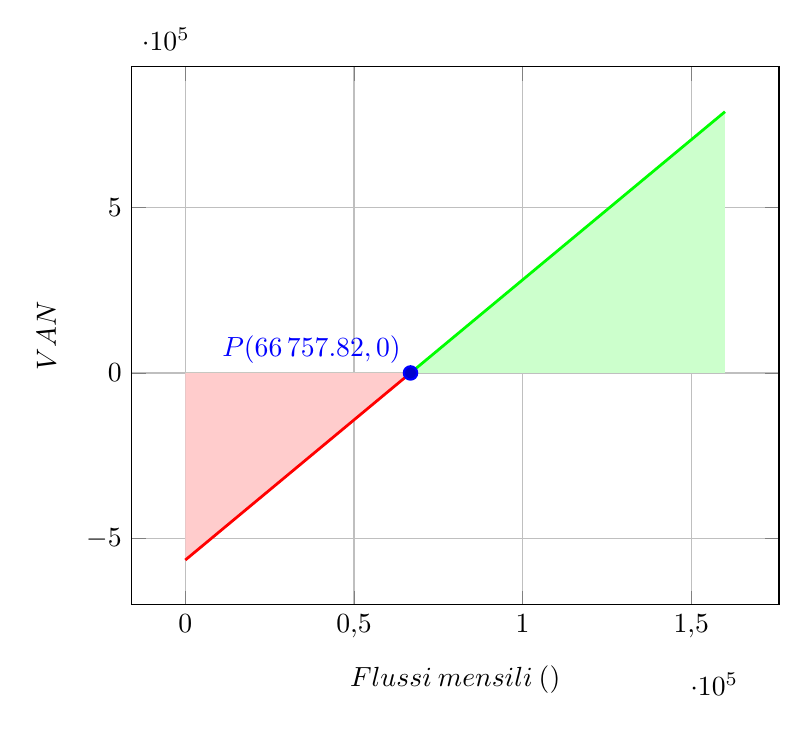
\begin{tikzpicture}[scale=1.2]
 \pgfkeys {
			/pgf/number format/.cd,
			set decimal separator={,{\!}},
			set thousands separator={}}

    \begin{axis}[thick,smooth, xlabel=$Flussi \: mensili \:(\mbox{\euro})$, ylabel=$VAN$, grid=major]    

		\addplot coordinates{( 66757.82, 0) };
							  
        \addplot+[domain=0:66757.82, name path=A,red,line width=1pt, no markers] {8.47654 * x - 565875.32};
        \addplot+[domain=66757.82:160000, name path=C,green,line width=1pt, no markers] {8.47654 * x - 565875.32};
        \addplot+[domain=0:160000, name path=B, draw=none,black, no markers] {0};

        \addplot[domain=0:66757.82, red!20] fill between[of=A and B];
        \addplot[domain=66757.82:160000, green!20] fill between[of=C and B];
        
        \coordinate[label=above left:\textcolor{blue}{$ P(66\thinspace 757.82,0)$}](a) at (66757.82,0);
    \end{axis}
\end{tikzpicture}
\newline
Da un punto di vista matematico, la (\ref{eq:van_caso_studio_2}) ammette come dominio tutto l'asse reale, ciò però \textit{fisicamente} non è possibile, perchè sarà vincolata \textit{a sinistra} dal valore del VAN in corrispondenza di $\mbox{\euro \: 0,00}$ flussi di entrate mensili (non è possibile avere entrate negative):  
	\begin{eqnarray}
	\label{eq:limite_sinistro}
 		y(0) & = & -565\thinspace 875,32 + 8,47654 \cdot 0 \nonumber \\
 								& = & -565\thinspace 875,32
	\end{eqnarray}
e come limite destro dal flusso di cassa mensile massimo raggiungibile $520\thinspace 865,39 \: \mbox{\euro}$ (corrispondenti a 8\thinspace 138,52 contratti):
	\begin{eqnarray}
	\label{eq:limite_superiore}
 		y(520\thinspace 865,39) & = & -565\thinspace 875,32 + 8,47654 \cdot 520\thinspace 865,39 \nonumber \\
 								& = & 3\thinspace 849\thinspace 260,99
	\end{eqnarray}
	
	\begin{tcolorbox}[colframe=blue!75!black,adjusted title=\textbf{Osservazione!}]
		Il \textbf{limite destro} è puramente teorico perchè si avrebbe nel caso in cui \underline{tutti} i potenziali clienti contattati stipulino alla fine il contratto del viaggio, situazione impossibile.
		\newline Il \textbf{limite sinistro}, invece, per quanto improbabile, può sempre verificarsi.
	\end{tcolorbox}	
in definitiva il dominio di (\ref{eq:van_caso_studio_2}) è pari a:
\[ Dom(y(x)) =	\left [ 0,00 ; 520\thinspace 865,39 \right)		\]
mentre il codominio di (\ref{eq:van_caso_studio_2}) è pari a:
\[ Codom(y(x)) =	\left [ -565\thinspace 875,32 ; 3\thinspace 849\thinspace 260,99 \right)		\]


%
%	Tabella relativa al caso teorico in cui non ci siano malati durante un anno
%
\begin{savenotes}
\begin{table}[htb]
\centering
 \caption{Variazione VAN}
 \begin{tabular}{p{3cm}D{,}{,}{5.2}D{,}{,}{5.2}D{,}{,}{5.2}D{,}{,}{7.4}}
 \toprule
 	& \multicolumn{1}{c}{Flusso di cassa mensile (\euro)} & \multicolumn{1}{c}{Contratti Mensili } &\multicolumn{1}{c}{\textbf{VAN (\euro)}}&\multicolumn{1}{c}{\textbf{ \% Contratti}} \\
 \midrule	
	\makebox[3cm][r]{Ottimo} & 520\thinspace 865,39 & 8\thinspace 138,52 & 3\thinspace 849\thinspace 260,99 & 1,0000\\
 	\rowcolor[gray]{.7} \makebox[3cm][r]{Pareggio} & 66\thinspace 757,82 & 1\thinspace 043,09 & 0,00 & 0,1282\\
 	\makebox[3cm][r]{Peggiore} &  0,00 & 0,00 & -565\thinspace 875,32 & 0,0000\\ 
 \bottomrule
 \end{tabular} 
\end{table}
\end{savenotes}

\subsection[Caso di Studio Realistico]{Caso di Studio Realistico}
\begin{savenotes}
\begin{table}[htb]
\centering
 \caption{Variazione VAN (Casi di Studio)}
 \begin{tabular}{p{3cm}D{,}{,}{5.2}D{,}{,}{5.2}D{,}{,}{5.2}D{,}{,}{7.4}}
 \toprule
 	& \multicolumn{1}{c}{Flusso di cassa mensile (\euro)} & \multicolumn{1}{c}{Contratti Mensili } &\multicolumn{1}{c}{\textbf{VAN (\euro)}}&\multicolumn{1}{c}{\textbf{ \% Contratti}} \\
 \midrule	
	\makebox[3cm][r]{Ottimo} & 520\thinspace 865,39 & 8\thinspace 138,52 & 3\thinspace 849\thinspace 260,99 & 1,0000\\
	\makebox[3cm][r]{Caso di Studio \# 2} & 104\thinspace 172,80 & 1\thinspace 627,70 & 317\thinspace 149,59 & 0,2000\\	
	 \rowcolor[gray]{.7} \makebox[3cm][r]{Caso di Studio} & 78\thinspace 129,81 & 1\thinspace 220,78 & 96\thinspace 395,14 & 0,1500\\
 	\makebox[3cm][r]{Pareggio} & 66\thinspace 757,82 & 1\thinspace 043,09 & 0,00 & 0,1282\\
 	\makebox[3cm][r]{Peggiore} &  0,00 & 0,00 & -565\thinspace 875,32 & 0,0000\\ 
 \bottomrule
 \end{tabular} 
\end{table}
\end{savenotes}



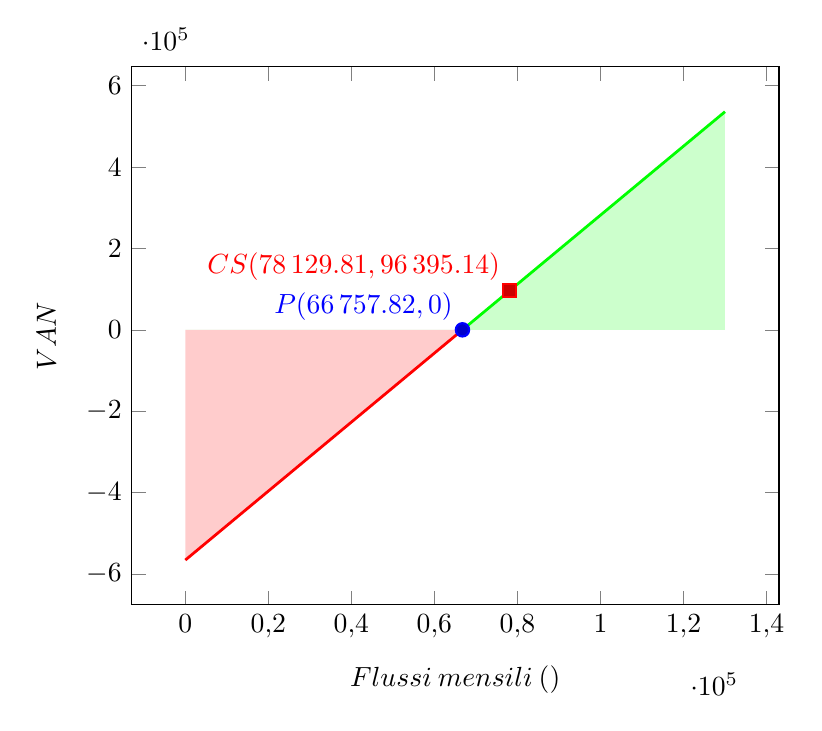
\begin{tikzpicture}[scale=1.2]
 \pgfkeys {
			/pgf/number format/.cd,
			set decimal separator={,{\!}},
			set thousands separator={}}

    \begin{axis}[thick,smooth, xlabel=$Flussi \: mensili \:(\mbox{\euro})$, ylabel=$VAN$]    

		\addplot coordinates{( 66757.82, 0) };
		\addplot coordinates{( 78129.81, 96395.14) };

        \coordinate[label=above left:\textcolor{blue}{$ P(66\thinspace 757.82,0)$}](a) at (66757.82,0);
        \coordinate[label=above left:\textcolor{red}{$ CS(78\thinspace 129.81,96\thinspace395.14)$}](a) at (78129.81,96395.14);        
							  
        \addplot+[domain=0:66757.82, name path=A,red,line width=1pt, no markers] {8.47654 * x - 565875.32};
        \addplot+[domain=66757.82:130000, name path=C,green,line width=1pt, no markers] {8.47654 * x - 565875.32};
        \addplot+[domain=0:130000, name path=B, draw=none,black, no markers] {0};

        \addplot[domain=0:66757.82, red!20] fill between[of=A and B];
        \addplot[domain=66757.82:130000, green!20] fill between[of=C and B];
    \end{axis}
\end{tikzpicture}

Considerando il fatturato mensile netto pari a $\mbox{\euro \: 78\thinspace 129,81}$, gli utili saranno pari a:
	\begin{equation}
	\label{eq:flussi_netti}
	\begin{split}
 		78\thinspace 129,81 \: \mbox{\euro} - \underbrace{60\thinspace 131,27 \: \mbox{\euro}}_{OPEX} = 17\thinspace 998,57 \: \mbox{\euro}	
 	\end{split}
	\end{equation}
fissando il tasso di sconto pari a (\ref{eq:wacc_tax_value}), si può osservare la seguente situazione:
%
%	Tabella relativa alla valutazione VAN = 0,00
%
\begin{savenotes}
\begin{table}[htb]
\centering
 \caption{VAN (Fatturato Mensile pari a $\mbox{\euro \:78\thinspace 129,81}$)}
 \begin{tabular}{p{5cm}D{,}{,}{7.2}D{,}{,}{7.2}D{,}{,}{7.2}}
 \toprule
 	\multicolumn{1}{c}{\textbf{Mese}} & \multicolumn{3}{c}{\textbf{Flussi di cassa (\euro)}} \\
 	& \multicolumn{1}{c}{Netti (\euro)} & \multicolumn{1}{c}{Attualizzati (\euro)} & \multicolumn{1}{c}{Totale (\euro)} \\
 \midrule
 	\makebox[5cm][r]{\textbf{Investimento Iniziale (CAPEX)}} & & & -56\thinspace 170,20 \\
 \midrule
 	\makebox[5cm][r]{Gennaio} & 17\thinspace 998,54 & 17\thinspace 011,85 & -39\thinspace 158,35\\ 
 	\makebox[5cm][r]{Febbraio} & 17\thinspace 998,54 & 16\thinspace 079,26 & -23\thinspace 079,09\\
 	\makebox[5cm][r]{Marzo} & 17\thinspace 998,54 & 15\thinspace 197,78 & -7\thinspace 881,31\\ 
 	\makebox[5cm][r]{Aprile} & 17\thinspace 998,54 & 14\thinspace 364,64 & 6\thinspace 483,33\\
 	\makebox[5cm][r]{Maggio} & 17\thinspace 998,54 & 13\thinspace 577,16 & 20\thinspace 060,49\\ 
 	\makebox[5cm][r]{Giugno} & 17\thinspace 998,54 & 12\thinspace 832,85 & 32\thinspace 893,34\\
 	\makebox[5cm][r]{Luglio} & 17\thinspace 998,54 & 12\thinspace 129,35 & 45\thinspace 022,69\\ 
 	\makebox[5cm][r]{Agosto} & 17\thinspace 998,54 & 11\thinspace 464,42 & 56\thinspace 487,11\\
 	\makebox[5cm][r]{Settembre} & 17\thinspace 998,54 & 10\thinspace 835,93 & 67\thinspace 323,04\\ 
 	\makebox[5cm][r]{Ottobre} & 17\thinspace 998,54 & 10\thinspace 241,90 & 77\thinspace 564,94\\
 	\makebox[5cm][r]{Novembre} & 17\thinspace 998,54 & 9\thinspace 680,44 & 87\thinspace 245,38\\ 
 	\makebox[5cm][r]{Dicembre} & 17\thinspace 998,54 & 9\thinspace 149,75 & 96\thinspace 395,13\\ 
 \bottomrule
 \end{tabular} 
\end{table}
\end{savenotes}
quindi si può osservare come già nel mese di Aprile riusciamo ad avere il \textbf{pareggio} con l'investimento iniziale!